\documentclass[a4paper, 12pt]{article}%тип документа

%%%Библиотеки
	%\usepackage[warn]{mathtext}	
	\usepackage[T2A]{fontenc} % кодировка
	\usepackage[utf8]{inputenc} % кодировка исходного текста
	\usepackage[english,russian]{babel} % локализация и переносы
	\usepackage{caption}
	\usepackage{listings}
	\usepackage{amsmath,amsfonts,amssymb,amsthm,mathtools}
	\usepackage{wasysym}
	\usepackage{graphicx}%Вставка картинок правильная
	\usepackage{float}%"Плавающие" картинки
	\usepackage{wrapfig}%Обтекание фигур (таблиц, картинок и прочего)
	\usepackage{fancyhdr} %загрузим пакет
	\usepackage{lscape}
	\usepackage{xcolor}
	\usepackage[normalem]{ulem}
	\usepackage{hyperref}

%%%Конец библиотек




%%%Настройка ссылок
	\hypersetup
	{
		colorlinks=true,
		linkcolor=blue,
		filecolor=magenta,
		urlcolor=blue
	}
%%%Конец настройки ссылок


%%%Настройка колонтитулы
	\pagestyle{fancy}
	\fancyhead{}
	\fancyhead[L]{Лабораторная работа}
	\fancyhead[R]{Талашкевич Даниил, группа Б01-009}
	\fancyfoot[C]{\thepage}
%%%конец настройки колонтитулы



							\begin{document}
						%%%%Начало документа%%%%


%%%Начало титульника
\begin{titlepage}

	\newpage
	\begin{center}
		\normalsize Московский физико-технический институт \\(госудраственный 			университет)
	\end{center}

	\vspace{6em}

	\begin{center}
		\Large Лабораторная работа по электричеству\\
	\end{center}

	\vspace{1em}

	\begin{center}
		\large \textbf{Резонанс напряжений в последовательном контуре [3.2.2]}
	\end{center}

	\vspace{2em}

	\begin{center}
		\large Талашкевич Даниил Александрович\\
		Группа Б01-009
	\end{center}

	\vspace{\fill}

	\begin{center}
	Долгопрудный \\2021
	\end{center}
	
\end{titlepage}
%%%Конец Титульника



%%%Настройка оглавления и нумерации страниц
	\thispagestyle{empty}
	\newpage
	\tableofcontents
	\newpage
	\setcounter{page}{1}
%%%Настройка оглавления и нумерации страниц


					%%%%%%Начало работы с текстом%%%%%%
		
\section{Аннотация}
\textbf{Цель работы:} исследование резонанса напряжений в последовательном
колебательном контуре с изменяемой ёмкостью, получение амплитудно­
частотных и фазово-частотных характеристик, определение основных па­
раметров контура.\\
\textbf{В работе используются:} генератор сигналов, источник напряжения,
нагрузкой которого является последовательный колебательный контур с
переменной ёмкостью, двухканальный осциллограф, цифровые вольтмет­
ры.



\subsection{Теоретическое вступление и модель}

\subsubsection{Вынужденные колебания}

Для схемы, изображенной ниже запишем правило Кирхгофа:

\begin{center}

    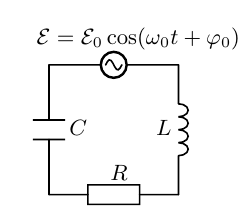
\includegraphics[scale=0.65]{pics/theory1.png} \\

\end{center}

\[
\ddot{U}_{C}+2 \gamma \dot{U}_{C}+\omega_{0}^{2} U_{C}=\omega_{0}^{2} \mathcal{E}_{0} \cos \left(\omega t+\varphi_{0}\right)
\]

Решая данное дифференциальное уравнение получаем:

\[ \boldsymbol{U}_{C}(t)=\boldsymbol{U}_{C 0} e^{i \omega t} \]

\[ \boldsymbol{U}_{C 0}=\frac{\mathcal{E}_{0}}{i \omega C Z}, \quad Z=R+i\left(\omega L-\frac{1}{\omega C}\right) \]

\[ \boldsymbol{I}_{0}=\frac{\mathcal{E}_{0}}{Z}, \quad \boldsymbol{U}_{R 0}=\frac{R \mathcal{E}_{0}}{Z}, \quad \boldsymbol{U}_{L 0}=i \omega L \frac{\mathcal{E}_{0}}{Z} \]

Т.е. закон Ома можно переписать в следующем виде:

\[ \boldsymbol{I}_{0}=\frac{\mathcal{E}_{0}}{Z}, \quad \boldsymbol{U}_{R 0}=Z_{R} \boldsymbol{I}_{0}, \quad \boldsymbol{U}_{C 0}=Z_{C} \boldsymbol{I}_{0}, \quad \boldsymbol{U}_{L 0}=Z_{L} \boldsymbol{I}_{0} , \text{ где}\]

\[ Z_{R}=R, \quad Z_{L}=i \omega L, \quad Z_{C}=\frac{1}{i \omega C} \]

Импедансы контура и его отдельных элементов -- комплексные числа -- могут быть представлены в показательной форме:

\[
Z=Z_{0} e^{i \psi}
\]

где $Z_{0}=|Z|-$ модуль комплексного числа, $\psi=\arg Z$ -- его аргумент (фаза). Для импеданса рассматриваемого последовательного контура при этом находим

\[
\begin{aligned}
Z_{0}=\sqrt{(\operatorname{Re} Z)^{2}+(\operatorname{Im} Z)^{2}} &=\sqrt{R^{2}+\left(\omega L-\frac{1}{\omega C}\right)^{2}}=\frac{R}{\cos \psi_{I}} \\
\operatorname{tg} \psi_{I} &=\frac{\operatorname{Im} Z}{\operatorname{Re} Z}=\frac{\omega L-\frac{1}{\omega C}}{R}
\end{aligned}
\]

Отсюда получаем выражения для действительной части тока и средней мощности активных потерь в контуре:

\[ I(t)=\frac{\mathcal{E}_{0}}{R} \cos \psi_{I} \cos \left(\omega t+\varphi_{0}-\psi_{I}\right) \]

\[ P=\left\langle I^{2} R\right\rangle=\frac{\mathcal{E}_{0}^{2}}{2 R} \cos ^{2} \psi_{I},\]

где угловые скобки означают усреднение по периоду колебаний.

\subsubsection{Резонанс}

Для исследования вынужденных колебаний и резонанса запишем вещественные части решений дифференциального уравнение, положив для сокраще­ния записи равной нулю начальную фазу: $\varphi_0$ = 0. В результате приходим к уравнениям

\[\begin{gathered}
I(t)=\frac{U_{R}(t)}{R}=I_{\omega} \cos \left(\omega t-\psi_{I}\right), \quad I_{\omega}=\frac{\mathcal{E}_{0}}{Z_{0}} \\
Z_{0}=R \sqrt{1+\left[\frac{\rho}{R}\left(\frac{\omega}{\omega_{0}}-\frac{\omega_{0}}{\omega}\right)\right]^{2}}, \quad \psi_{I}=\operatorname{arctg}\left[\frac{\rho}{R}\left(\frac{\omega}{\omega_{0}}-\frac{\omega_{0}}{\omega}\right)\right] \\
U_{C}(t)=U_{C \omega} \cos \left(\omega t-\psi_{C}\right), \quad U_{C \omega}=\mathcal{E}_{0} \frac{\rho}{Z_{0}} \frac{\omega_{0}}{\omega}, \quad \psi_{C}=\psi_{I}+\pi / 2, \\
U_{L}(t)=U_{L \omega} \cos \left(\omega t-\psi_{L}\right), \quad U_{L \omega}=\mathcal{E}_{0} \frac{\rho}{Z_{0}} \frac{\omega}{\omega_{0}}, \quad \psi_{L}=\psi_{I}-\pi / 2 .
\end{gathered}\]

2) Поведение системы носит резонансный характер: при $\omega=\omega_{0}$, когда мнимая часть импеданса контура $\operatorname{Im} Z=0$ и соответственно

\[
\omega_{0} L=\frac{1}{\omega_{0} C}=\rho, \quad \operatorname{Im} Z=0, \quad Z_{0}=R, \quad \psi_{I}=0
\]

амплитуды тока и напряжения на сопротивлении $R$ достигают максимальных значений:

\[
I_{\omega_{0}}=\mathcal{E}_{0} / R, \quad U_{R \omega_{0}}=R I_{\omega_{0}}=\mathcal{E}_{0}
\]

\[
I_{\omega}=\frac{\mathcal{E}_{0} / R}{\sqrt{1+(\tau \Delta \omega)^{2}}}, U_{C \omega}=\frac{Q \mathcal{E}_{0} \omega_{0} / \omega}{\sqrt{1+(\tau \Delta \omega)^{2}}}, U_{L \omega}=\frac{Q \mathcal{E}_{0} \omega / \omega_{0}}{\sqrt{1+(\tau \Delta \omega)^{2}}}
\]

В резонансе, когда для высокодобротного контура $\omega=\omega_{0}, \Delta \omega=0$, выражения для амплитуд тока и напряжений на ёмкости и индуктивности, фазовых сдвигов $\psi$ и их производных по частоте 

$\psi^{\prime}=d \psi / d \omega$ принимают вид

\[
\begin{gathered}
I_{\omega}\left(\omega_{0}\right)=\frac{\mathcal{E}_{0}}{R}, \quad \psi_{I}\left(\omega_{0}\right)=0 \\
U_{C \omega}\left(\omega_{0}\right)=Q \mathcal{E}_{0}, \quad \psi_{C}\left(\omega_{0}\right)=\frac{\pi}{2} \\
U_{L \omega}\left(\omega_{0}\right)=Q \mathcal{E}_{0}, \quad \psi_{L}\left(\omega_{0}\right)=-\frac{\pi}{2} \\
\psi_{I}^{\prime}\left(\omega_{0}\right)=\psi_{L}^{\prime}\left(\omega_{0}\right)=\psi_{C}^{\prime}\left(\omega_{0}\right)=\tau
\end{gathered}
\]

Для параллельного контура можно получить выражения для аналогичных величин:

\[
\begin{aligned}
&I_{C}(t)=Q I_{0} \frac{\omega}{\omega_{0}} \frac{\cos \left(\omega t-\psi_{C}\right)}{\sqrt{1+(\tau \Delta \omega)^{2}}}, \quad \psi_{C}=\operatorname{arctg}(\tau \Delta \omega)-\frac{\pi}{2}+\frac{1}{Q} \\
&I_{L}(t)=Q I_{0} \frac{\omega_{0}}{\omega} \frac{\cos \left(\omega t-\psi_{L}\right)}{\sqrt{1+(\tau \Delta \omega)^{2}}}, \quad \psi_{L}=\operatorname{arctg}(\tau \Delta \omega)+\frac{\pi}{2} \\
&U(t)=Q \rho I_{0} \frac{\cos \left(\omega t-\psi_{U}\right)}{\sqrt{1+(\tau \Delta \omega)^{2}}}, \quad \psi_{U}=\operatorname{arctg}(\tau \Delta \omega)+\frac{\omega_{0}}{\omega} \frac{1}{Q}
\end{aligned}
\]

При резонансе, когда в принятом выше приближении $\omega=\omega_{0}, \Delta \omega=0$, амплитуды токов в ветвях контура, напряжения на нём, фазовые сдвиги $\psi$ и их производные по циклической частоте $\psi^{\prime}=d \psi / d \omega$ принимают вид

\[
\begin{gathered}
I_{C \omega}\left(\omega_{0}\right)=Q I_{0}, \quad \psi_{C}\left(\omega_{0}\right)=-\frac{\pi}{2}+\frac{1}{Q} \\
I_{L \omega}\left(\omega_{0}\right)=Q I_{0}, \quad \psi_{L}\left(\omega_{0}\right)=\frac{\pi}{2} \\
U_{\omega}\left(\omega_{0}\right)=Q^{2} R I_{0}, \quad \psi_{U}\left(\omega_{0}\right)=\frac{1}{Q} \\
\psi_{C}^{\prime}\left(\omega_{0}\right)=\psi_{L}^{\prime}\left(\omega_{0}\right)=\psi_{U}^{\prime}\left(\omega_{0}\right)=\tau
\end{gathered}
\]

\subsection{Экспериментальная установка}

В данной работе изучаются резонансные явления в последовательном колебательном контуре (резонанс напряжений). Схема экспериментального стенда показана на рис. $1 .$ Синусоидальный сигнал от генератора поступает на вход управляемого напряжсением источника напрялсения (см., например, [3]), собранного на операционном усилителе, питание которого осуществляется встроенным блоком-выпрямителем от сети $\sim 220 \mathrm{~B}$ (цепь питания на схеме не показана). Источник напряжсения (источник с нулевым внутренним сопротивлением) обеспечивает с высокой точностью постоянство амплитуды сигнала $\mathcal{E}=\mathcal{E}_{0} \cos \left(\omega t+\varphi_{0}\right)$ на меняющейся по величине нагрузке - последовательном колебательном контуре, изображённом на рис. 1 в виде эквивалентной схемы.

Источник напряжения, колебательный контур и блок питания заключены в отдельный корпус, отмеченный на рисунке штриховой линией. На корпусе имеются коаксиальные разъёмы «Вход», «$U_1$» и «$U_{2}$», а также переключатель магазина ёмкостей $C_{n}$ с указателем номера $n=1,2, \ldots$ 7. Величины ёмкостей $C_{n}$ указаны на установке. Напряжение $\mathcal{E}$ на контуре через разъём «$U_1$» попадает одновременно на канал 1 осциллографа и вход 1-го цифрового вольтметра. Напряжение на конденсаторе $U_{C}$ подаётся через разъём «$U_2$» одновременно на канал 2 осциллографа и вход 2-го цифрового вольтметра.

\begin{center}

    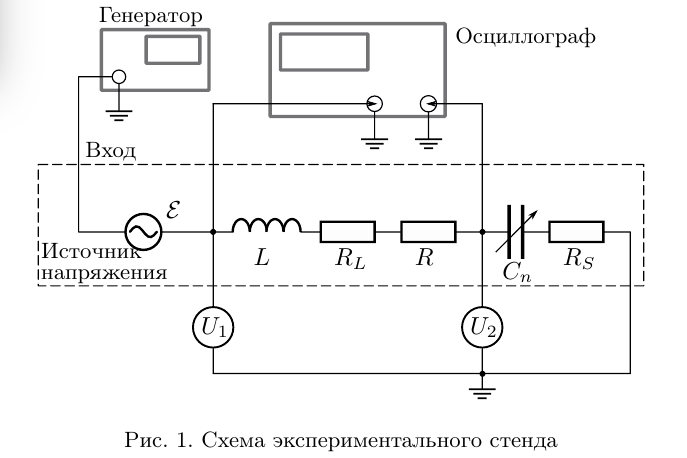
\includegraphics[scale=0.65]{pics/scheme1.png} \\
   % \textit{Рис. 1. Схема установки}

\end{center}

\section{Ход работы}

\subsection{Закон Ома в цепи переменного тока}

Подготовив установку, выставив пределы всех измерительных приборов и выкрутив ручку регулятора напряжения в положение напряжения $\approx 127 B$, можем проступать к снятию данных.

Указатель на положение сердечника установили на отметку $x = 5 \pm 1 \text{ мм} $ и, перемещая сердечник шагами по 2 мм, снимаем зависимость тока $I$, напряжения $U_R, U_L, U_{R+L}$, а так же мощности $P_L$ от координаты сердечника $x$.

Полученные результаты представлены в таблице.

\begin{table}[!h]
\begin{tabular}{|c|c|c|c|c|c|c|c|c|}
\hline 
  & $x, \text{ мм}$ & $U_R, B$ & $U_{R+L}, B$ & $U_L, B$ & $I, \text{ дел}$ & $I,\ A$ & $P_L,\text{ дел}$ & $P_L,\text{ Вт}$ \\ 
\hline 
1 & 5 & 73 & 112 & 73 & 34 & 85 & 42 & 10.5 \\ 
\hline 
2 & 7 & 78 & 110 & 65 & 36 & 90 & 38 & 9.5 \\ 
\hline 
3 & 9 & 81 & 109 & 61 & 37 & 92.5 & 36 & 9 \\ 
\hline 
4 & 11 & 84 & 108 & 56 & 37.5 & 93.75 & 34 & 8.5 \\ 
\hline 
5 & 13 & 85 & 107 & 52 & 39.5 & 98.75 & 32 & 8 \\ 
\hline 
6 & 15 & 87 & 107 & 50 & 40 & 100 & 31 & 7.75 \\ 
\hline 
7 & 17 & 89 & 107 & 47 & 41 & 102.5 & 30 & 7.5 \\ 
\hline 
\end{tabular} 
\caption{Показания приборов от положения сердечника}
\end{table}

Так же для снятия и обработки результатов пригодилась таблица с характеристиками приборов.

\begin{table}[!h]
\begin{center}
\begin{tabular}{|c|}
\hline 
$\text{Амперметр} - 2.5\ A$ \\ 
\hline 
$\text{Вольтметры} - 150\ B$ \\ 
\hline 
$\text{Ваттметр}   - 25\ Bт$ \\ 
\hline 
$\text{Переключатель катушки напряжений} - 100\ B$ \\ 
\hline 
$\text{Штепсель токовой катушки I} - 0.25\ A$ \\ 
\hline 
$R_1 - 98 \text{ Ом}$ \\ 
\hline 
\end{tabular} 
\caption{Характеристики установки}
\end{center}
\end{table}

\subsection{Резонанс напряжений}

Подготовим установку вместе с измерительными приборами. Установив сердечник в среднее положение ($x \approx 12 \text{ мм}$), подбираем значение ёмкости так, чтобы наблюдать резонанс тока по изменению эллипса на экране ЭО.

При резонанс измерим показания $I, U_{C,\text{рез}}, U_{\sum,\text{рез}}$ и по полученным данным оценим добротность контура по формуле (10).

\begin{table}[!h]
\begin{center}
\begin{tabular}{|c|c|c|c|c|c|c|}
\hline 
$x,\text{ мм}$ & $C,\text{ мкФ}$ & $I,\ A$ & $U_C, B$ & $U_{\sum}\ B$ & $Q$ & $R_{\text{доп}}$ \\ 
\hline 
12 & 55.2 & 410 & 242 & 41 & 5.902 & 5.6 \\ 
\hline 
\end{tabular}
\caption{Показания приборов при резонансе}
\end{center} 
\end{table}

Для резонансного положения сердечника измерим омическое сопротивление витков каткушки с помощью мультиметра $GDM$, а затем -- $L$, $r_L$ с помощью измерителя $LCR$ на частотах 50 Гц и 1 кГц.


\begin{table}[!h]
\begin{center}
\begin{tabular}{|c|c|}
\hline Для 50 Гц &\\
\hline $\mathrm{L}, $ мН& $159,42 $\\
\hline $\mathrm{r_L}, $ Ом& 3,696\\
\hline Для 1 КГц &\\
\hline $\mathrm{L}, $ мН& $141,58 $\\
\hline $\mathrm{r_L}, $ Ом& 52,97\\
\hline
\end{tabular}
\caption{Данные с мультиметра $GDM$ и $LCR$ измерителя}
\end{center} 
\end{table}


\section{Обработка результатов}

\begin{itemize}

\item По результатам измерений $P_L$ и $I$ найдем значение $r_L$ по следующей формуле $P_L = I^2r_L $. Теперь по следующей формуле 

\begin{equation}
U_L = I \sqrt{r_L^2 + (\Omega L)^2}
\end{equation}

вычислим $L$ ($\Omega = 50$ Гц).

Результаты вычислений заносим в таблицу:


\begin{table}[!h]
\begin{center}
\begin{tabular}{|c|c|c|}
\hline $r_L$, Ом & $x$, мм & $L$, Гн\\
\hline 1,45 & 5 & 0,01718 \\
\hline 1,17 & 7 & 0,01444 \\
\hline 1,05 & 9 & 0,01319 \\
\hline 0,97 & 11 & 0,01195 \\
\hline 0,82 & 13 & 0,01053 \\
\hline 0,78 & 15 & 0,01 \\
\hline 0,71 & 17 & 0,00917 \\
\hline
\end{tabular}
\end{center} 
\end{table}


Построим графики зависимостей $L$ и $r_L$ от положения сердечника и по полученной аппроксимации зависимости определем по ним значения $L$ и $r_L$, соответствующие резонансному положению сердечника.

%\newpage

\begin{center}

\begin{figure}[!h]
	\center{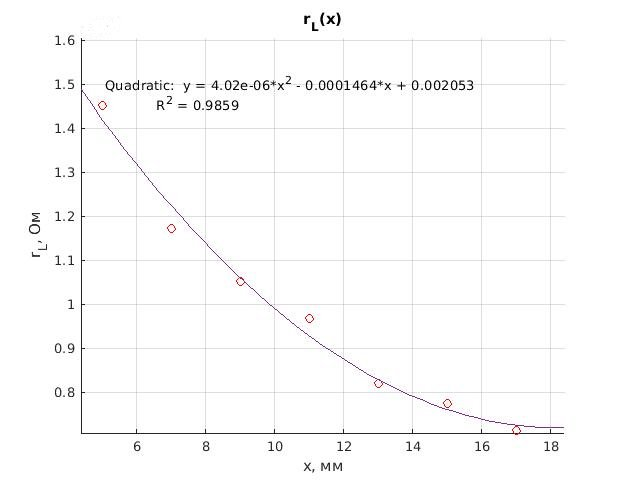
\includegraphics[scale=0.4]{pics/graph1_quad_fff.jpg}}
\end{figure}

\begin{figure}[!h]
	\center{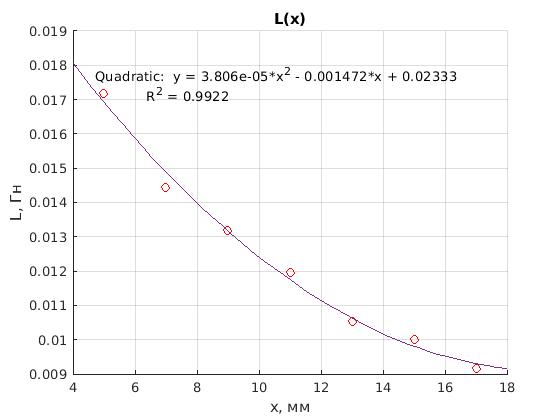
\includegraphics[scale=0.5]{L(x)_smakk.jpg}}
\end{figure}

\end{center}


\item  Рассчитаем активное сопротивление катушки $r_L$ через ток и напряжение
на контуре, используя следующие соотношения:

\[  R_{\Sigma}=R_1 + r_{L} \]

\[  U_{\Sigma, \text{ рез}}=I_{\text{ рез}} R_{\Sigma}, \quad U_{C, \text { рез }}=\frac{I_{\text{ рез}}}{\Omega C} \]

Тогда получаем	

\[r_L = \frac{U_{\Sigma, \text{ рез}}}{U_{C, \text { рез }} \cdot \Omega C} - R_1 = 1,16 \text{ Ом}\]

Так же рассчитаем $L$ и $r_L$ через добротность $Q$ при помощи следующих соотношений 

\[ \omega_{0} L=\frac{1}{\omega_{0} C} \]

\[ Q=\frac{\omega_{0} L}{R_{\Sigma}}=\frac{1}{\omega_{0} C R_{\Sigma}} \]

\[ R_{\Sigma}=R_1 + r_{L} \]

\[ Q=\frac{U_{C, \text{ рез}}}{U_{\Sigma, \text{ рез}}}\]

Отсюда получаем $L = 120,32$; $r_L = 1,08 \text{ Ом}$.

\item Сведем результаты измерений в таблицу:

\begin{table}[!h]
\begin{center}
\begin{tabular}{|c|c|c|c|c|c|}
\hline & Омметр & $LCR$ & График  & $f\left(I, U_{\Sigma}\right)_{\text{рез}}$ & $f(Q)$ \\
\hline \hline$r_{L}$, Ом & 2,170 &3,70 & 0,88 & 1,16 & 1,08 \\
$L$, мГн & $-$ & 159,42 & 111,47 & $-$ & 120,32\\
\hline
\end{tabular}
\caption{Данные с мультиметра $GDM$ и $LCR$ измерителя}
\end{center} 
\end{table}

\end{itemize}


\section{Вывод}

При выполнении данной лабораторной работы было получено, что разные методы дают величины одного порядка, различающиеся в пределах прогрешност между собой. Однако не все они попадают в пределах погрешности с действительной величиной. Причиной этого может являться эффект, при котором катушка и конденсатор имеют ненулевую действительную часть импиданса, в связи с чем происходят потери еще и на этих элементах и теоретическая зависимость будет иметь другой характер.

\section{Литература}

\begin{enumerate}
\item \textbf{Лабораторный практикум по общей физике:} Учебное пособие. В трех томах. Т. 2. Электричество и магнетизм /Гладун А.Д., Александров Д.А., Берулёва Н.С. и др.; Под ред. А.Д. Гладуна - М.: МФТИ, 2007. - 280 с.
\end{enumerate}		
		
					
\end{document}